
% I scanned through a lot of the cites quickly, but I might have made mistakes while describing their results. I've commented on specific papers that I had a bit of trouble understanding, and we'd have to take a closer look in the final draft.

Approximate convex hulls are very useful because they give a good estimate of the boundary of a set of points, often using much less space than the true convex hull. In most cases where the true convex hull is used, we can tolerate some error, and so we can use an approximation instead. Direct applications of such boundary approximations include surface simplification~\cite{Heckbert97surveyof}, but they also play an important role in coresets and non-negative matrix factorization.
% Check the surface simplification reference more carefully, it seems to be true, but

\section{Coresets}

Given a set of points $P \subseteq \mathbb{R}^n$, we might be interested in some property of the set, $\mu(P)$. For example, we might want to know the volume of the smallest sphere containing $P$. More precisely, $\mu$ is a map from $\mathbb{R}^n$ to $\mathbb{R}^+ \cup \{0\}$, and is monotone, that is, if $P_1 \subseteq P_2$ then $\mu(P_1) \leq \mu(P_2)$.

\begin{definition}
An $\epsilon$-coreset~\cite{Agarwal:2004:AEM:1008731.1008736,survey}, $S \subseteq P$ gives us an approximation of $\mu(P)$, where $\epsilon > 0$. In particular, $(1-\epsilon)\mu(P) \leq \mu(S) \leq \mu(P)$. 
\end{definition}

The general principles behind coresets are used in machine learning~\cite{cvms, peled-application, Feldman:2011:STM:2986459.2986698, Feldman, icml2015_bachem15}, robotics~\cite{6907021}, clustering~\cite{Har-Peled:2004:CKK:1007352.1007400}, and many other areas of research.

\subsection{$\epsilon$-kernels}

One of the most important types of coresets is the $\epsilon$-kernel~\cite{Agarwal:2004:AEM:1008731.1008736,survey}, because it is a coreset for many properties $\mu$.

\begin{definition}
Given a set of points $P \subseteq \mathbb{R}^d$ and $u \in \mathbb{R}^d$ with $|u|_2 = 1$, the \emph{directional width} of $P$ in direction $u$ is given by,
\[ \omega(u, P) = \max_{p \in P}\langle p, v \rangle - \min_{p \in P}\langle p, v \rangle \] 
\end{definition}

\begin{definition}
A subset $Q$ of $P$ is called an $\epsilon$-kernel of $P$ if for all $u$ with $|u|_2 = 1$,
\[ (1 - \epsilon) \omega(u, P) \leq \omega(u, Q) \]
\end{definition}

In both the batch and streaming setting, algorithms to find an $\epsilon$-kernel almost always reduce to finding an $\epsilon$-approximate convex hull of a set of points contained in the unit sphere. Most of these algorithms also assume that the dimension $d$ is a constant (so even a $d^d$ multiplicative term in the time or space complexity is ignored).
\\

$\epsilon$-kernels are used in a wide range of applications. For example, Barequet and Har-Peled~\cite{BAREQUET200191} explain how $\epsilon$-kernels can be used to efficiently approximate the minimum volume bounding box containing a set of points. Minimum volume bounding boxes are used in computer graphics (for fast scene rendering and collision detection), and statistics (for range queries on samples)~\cite{BAREQUET200191}. Agarwal, Har-Peled, and Varadarajan~\cite{Agarwal:2004:AEM:1008731.1008736} explain how $\epsilon$-kernels can also be used to find the minimum width cylinderical shell, and the minimum width sphere, containing a set of points. $\epsilon$-kernels can also be used to approximate k-regret minimizing sets~\cite{DBLP:journals/corr/AgarwalKSS17}.

\subsection{Batch Algorithms for $\epsilon$-kernels}

In the batch setting, Bentley, Preparata, and Faust~\cite{Bentley:1982:AAC:358315.358392} give a $1/\epsilon^{d-1}$ space algorithm for computing an $\epsilon$-approximate convex hull of a set of points. Agarwal, Har-Peled, and Varadarajan~\cite{Agarwal:2004:AEM:1008731.1008736} use this to give a $1/\epsilon^{d-1}$ space algorithm for computing an $\epsilon$-kernel. This was improved to a $1/\epsilon^{\frac{d-1}{2}}$ space algorithm~\cite{Yu:2004:PMS:997817.997858, CHAN200620} for computing an $\epsilon$-kernel. The time bounds on these algorithms were further improved~\cite{timchansocg2017, aryasocg2017}. All of these methods involve computing the $\epsilon$-approximate convex hull.
\\
% Confirm that Agarwal, Har-Peled, and Varadarajan's original algorithm is 1/eps^(d-1) and not 1/eps^((d-1)/2)
% Cinfirm that all timchansocg2017 and aryasocg2017 did was improve the time bound, and not the space bound.

Ignoring specific details about the point set $P$, the space usage of $1/\epsilon^{\frac{d-1}{2}}$ is optimal: there exists some set of points $P$ where the $\epsilon$-approximate convex hull (and the $\epsilon$-kernel) must store $1/\epsilon^{\frac{d-1}{2}}$ points.
\\

However, in many cases, the $\epsilon$-approximate convex hull is much smaller than $1/\epsilon^{\frac{d-1}{2}}$. For example, suppose we have points $p_1, p_2, p_3$ in high dimensional space. We generate data points by taking convex combinations of $p_1, p_2, p_3$, and then perturbing the generated point by $\epsilon$. Suppose we give the algorithm a set of points $P$ containing $p_1, p_2, p_3$ and the generated data points. The $\epsilon$-approximate convex hull of this set has size at most 3 (it suffices to keep $p_1, p_2, p_3$), and it would be wasteful to store $1/\epsilon^{\frac{d-1}{2}}$ points especially when $d$ is large. Blum, Har-Peled, and Raichel~\cite{blum-peled} give the only known algorithms for $\epsilon$-approximate convex hulls that are competitive with the optimal of the given point set.

\subsection{Streaming Algorithms for $\epsilon$-kernels}

In many cases, the point set might be much larger than the amount of memory available (for example in financial markets, packet flow monitors, sensor networks)~\cite{Hershberger:2004:ASG:1055558.1055595}. In these cases we want a streaming (one pass) algorithm that sees each point exactly once, and has low memory consumption.
\\

Hershberger and Suri give a 2D streaming algorithm for $\epsilon$-approximate convex hulls that uses $1/\sqrt{\epsilon}$ space~\cite{Hershberger:2004:ASG:1055558.1055595}. Agarwal, Har-Peled, and Varadarajan~\cite{Agarwal:2004:AEM:1008731.1008736} give a streaming algorithm for $\epsilon$-kernels that uses $(1/\epsilon^{\frac{d-1}{2}})\log^d{n}$ space. Chan removes the dependency on $n$ and gives a streaming algorithm for $\epsilon$-kernels that uses $(1/\epsilon^{d-3/2})\log^d{1/\epsilon}$ space~\cite{CHAN200620}. This was then improved to $(1/\epsilon^{\frac{d-1}{2}})\log{1/\epsilon}$~\cite{Zarrabi-Zadeh:2011:ASS:1967334.1967341} and the time complexity was further improved by Arya and Chan~\cite{Arya:2014:BOA:2582112.2582161}. Chan also gives a streamling algorithm based on polynomial methods~\cite{chansocg2016}. All of these methods involve clever tricks and transformations, but a core part of these methods is a streaming algorithm to maintain an $\epsilon$-approximate convex hull of a set of points.
\\
% How is Agarwal, Har-Peled, and Varadarajan's streaming algorithm 1/eps^((d-1)/2), something is fishy.

Like in the batch case, if we ignore the particular point set $P$ we are dealing with, a space usage of $\frac{1}{\epsilon^{(d-1)/2}}$ is optimal. However, in many cases we can do much better. In this work our aim is to come up with streaming algorithms that are competitive with the optimal $\epsilon$-approximate convex hull of the given point set. To our knowledge there is no existing work of this kind.

\section{Matrix Factorization}

Matrix factorization is a popular technique in unsupervised machine learning.

\subsection{Non-Negative Matrix Factorization (NMF)}

In classical non-negative matrix factorization (NMF) we are given $n$ data points, with non-negative coordinates, in $d$ dimensional space. We want to find a minimal collection $T$ of topics with non-negative coordinates such that every data point can be represented as a non-negative linear combination of the topics in $T$. In approximate non-negative matrix factorization the data points should be approximately representable (based on some distance metric) as a non-negative linear combination of the topics in $T$. 
\\

Non-negative matrix factorization decomposes objects into parts comprising those objects. For example, Lee and Seung use NMF ~\cite{leeseung95} to represent images of faces as combinations of parts in those faces, as shown in figure~\ref{fig:image-nmf}.

\begin{figure}[!ht]
\centering
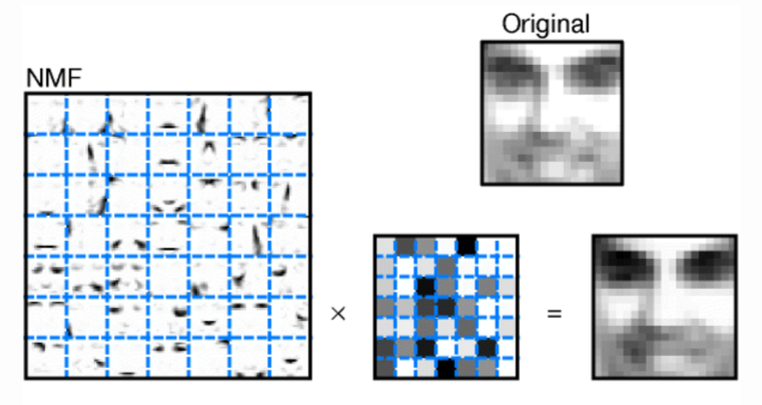
\includegraphics[scale=0.3]{image-nmf}
\caption{The boxes on the left represent parts of the face that are summed together to approximate the face}
\label{fig:image-nmf}
\end{figure}

Lee and Seung also used NMF to find out what topics encyclopedic articles are about ~\cite{leeseung95}. For example, the encyclopedic entry `constitution of the United States' was decomposed into a topic represented by the words (`court', `government', `council', `culture', `supreme', ...) and a topic represented by the words (`president', `served', `governer', `secretary', `senate', ...). NMF has a wide range of applications. For example, NMF is used for text mining~\cite{Berry2005, Murphy2012LearningEA}, speech de-noising~\cite{schmidt-noise}, and energy disaggregation~\cite{Kolter:2010:EDV:2997189.2997318}.
\\

Related matrix factorization methods, like PCA, allow negative weights. While PCA has many important uses, NMF gives a better parts based decomposition~\cite{leeseung95}. This is because a lot of data, like audio signals, is built up from a non-negative sum of of signals, for example we might add the sound of birds chirping to the sound of leaves rustling in the wind. Allowing negative weights could lead to complex cancellations which lead to a less intuitive representation. For example, natural audio signals do not typically involve subtracting the sound of birds chirping, and images of faces do not involve subtracting a nose from a face.

\subsection{Algorithms for NMF}

Stated more formally, in NMF we are given a $d-$by$-n$ matrix $A$ where the columns are data points. We want to find the smallest $d-$by$-t$ topic matrix $T$ where the columns represent topics, and a $t-$by$-n$ weights matrix $W$ where the columns represent weights s.t. $A = TW$. In some formulations~\cite{leeseung95}, entries of $A$, $T$, and $W$ are non-negative, in some formulations only the weights matrix $W$ is required to be non-negatvie~\cite{NIPS2016_6417}. In approximate NMF, we are given a distance metric $d$ and a distance $\epsilon$ and want to find the smallest $T$ s.t. $d(A,TW) < \epsilon$. Alternatively, we are given $k$ and a norm $|\cdot|$, and want to minimize $|A-TW|$, where $T$ has $k$ columns.
\\

NMF is NP-complete ~\cite{nmf-np-complete}, so most approaches focus on finding approximation algorithms or solving NMF for certain classes of problems. Lee and Seung use a multiplicative update rule and show that their approach converges to a local optimum ~\cite{Lee00algorithmsfor}. Alternatively, it can be shown for common distance metrics that the optimization problem is convex if we fix $T$ or $W$. Lin uses this to alternate between optimizing $T$ and $W$ using gradient descent, and shows that this converges to a local optimum ~\cite{lin-grad-optimization}. 
\\

Donoho and Stodden introduce a condition called separability~\cite{NIPS2003_2463}: $A$ is separable if each column contains some row which is $1$ only in that column. For example, if each article in a collection has an `anchor' word that is unique to the article then the collection is separable. Arora et al prove an efficient polynomial time algorithm for separable NMF ~\cite{DBLP:arora} and show that separable NMF works well in practice~\cite{DBLP:arora-practice}. More recent research focuses on near separability~\cite{Gillis:2014:RNN:2627435.2638575}.

\subsection{Sparse Coding}

 The number of topics is often large. Instead of simply finding the smallest topic matrix $T$ such that $A = TW$, we might want to find $T$ so that every data point can be represented (or approximately represented) as the sum of a small number of topics (for example, at most $k$ topics). This problem is known as \emph{sparse NMF} or \emph{non-negative sparse coding}. Clustering requires every data point to be approximately represented by exactly one topic in $T$.
 \\
 
Intuitively, sparsity is appealing because objects tend to be made up of a small number of parts. Another way of looking at this is that without sparsity, we might overfit the topics to the data. In particular, if we have $n >> d$ points in $d$ dimensional space, we can simply pick a unit vector along each axis as our topics. Every data point can be represented as a non-negative combination of these vectors, but this representation does not reveal any structure about the data.
\\

In some cases, NMF naturally gives a sparse representation. Lee and Seung show that NMF learns a sparse representation of facial images~\cite{leeseung95}. A combinatorial analogy for this is: suppose a human face is built up from a sum of 5 different types of noses, 5 different types of eyes, and 5 different types of mouths. There are 125 possible faces, which represent combinations of these parts. A non-negative matrix factorization with 15 topics is forced to learn the 5 noses, 5 eyes, and 5 mouths that add up to the face in order to give a compact representation.
\\

However, in some cases NMF does not give a meaningful or sparse representation, and the degree of sparsity in NMF cannot be tuned~\cite{hoyer-nmf}. Sparse NMF, which is related to sparse coding, adds additional constraints to incentivize sparsity. Many algorithms for sparse NMF simply use $L_1$ or $L_2$ regularization on the weights matrix $W$~\cite{Lee97unsupervisedlearning, Berry2005, Mairal:2010:OLM:1756006.1756008, Murphy2012LearningEA}. There has been a lot of research on sparse NMF. Hoyer gives an algorithm for sparse NMF and shows that it performs well on an image database~\cite{hoyer-nmf}. Schmidt, Larsen, and Hsiao use sparse NMF to separate wind noise from audio tracks~\cite{schmidt-noise}. 

\subsection{The Approximate Convex Hull Approach}

It turns out that $\epsilon$-approximate convex hulls can be used for sparse NMF~\cite{blum-peled}. In particular, suppose we normalize the columns of $A$ so that they lie in the unit sphere (for example by normalizing the $L_1$ or $L_2$ norm of each column to be 1). Let $T$ be a matrix where the columns correspond to an $\epsilon$-approximate convex hull (of the columns of $A$) of minimal size. Then, for all columns $A_i$ in $A$, there exists a convex combination $w$ such that $|A_i - Tw|_2 \leq \epsilon$. So this gives us a non-negative matrix factorization (on a different norm).
\\

Furthermore, we get a sparsity guarantee. In particular, for all culumns $A_i$ in $A$, there exists a convex combination $w$ with at most $1/\epsilon^2$ non-zero elements such that $|A_i - Tw|_2 \leq 2\epsilon$~\cite{Har-Peled:2016:SEV:2984951.2984998, blum-peled}.
\\

The hyperspectral unmixing literature often works with non-negative matrix factorizations where the data points are scaled to have the same $L_1$ norm, and the weights are restricted to be convex. However, the topics are usually not restricted to come from the data points, their algorithms typically ensure that the topics form a simplex, and they use different error measures and regularization functions~\cite{6200362, gillis_survey}. More experiments would need to be done to see if our approch can be used for hyperspectral unmixing.
\\
% Verify that the hyperspectral unmixing paper scales to L1 norm. Their figures strongly suggest this, but they don't describe this.

Arora, Ge, Kannan, and Moitra, also scale the data points to have the unit $L_1$ norm. They explain that if we do this scaling then without loss of generality we can assume the weights are convex~\cite{Arora:2012:CNM:2213977.2213994, moitramonograph}. Lee and Seung suggest using convex weights and show that this gives better results in a USPS digit classification dataset, however in reality they use $L_2$ regularization to approximate the convexity constraint~\cite{Lee97unsupervisedlearning}. The main difference between these models and ours is that they use the Frobenius norm, whereas we ensure that all data points are within distance $\epsilon$ from the approximate convex hull. We might get more provable guarantees because of our stronger requirement, but our algorithms might be more sensitive to noise or might need a preprocessing step to get rid of noise. Additionally, we restrict our topics to be data points (that is, each column of $T$ is a column of $A$).
\\

We follow the experimental setup in~\cite{Lee97unsupervisedlearning} to test the assumptions of our model. We use the MNIST classification task. Our preliminary experiments (see Appendix A) show that for large topic matrices, using an approximation algorithm to find an $\epsilon$-approximate convex hull (described in~\cite{blum-peled}) outperforms using Matlab's non-negative matrix factorization method. While these experiments are not thorough, they suggest that our modeling differences from other papers in the NMF literature might be reasonable.

